\section{Experimentos}

\subsection{Actividad 1: Cambio de color de fondo (glClearColor)}
Para resolver este primer ejercicio, el objetivo fue aplicar una paleta de cinco colores específicos al fondo de nuestra ventana de renderizado. Dado que OpenGL trabaja con valores flotantes normalizados entre 0.0 y 1.0 en lugar del formato hexadecimal tradicional, el primer paso de la implementación fue realizar la conversión matemática de los colores solicitados dividiendo sus valores RGB entre 255.\\

Una vez obtenidos los porcentajes de intensidad para cada canal (rojo, verde y azul), trabajamos directamente sobre el código fuente en el archivo \texttt{01\_IntroOpenGL.cpp}. Nos enfocamos en la función \texttt{keyboardCallback}, que es la encargada de manejar las interrupciones generadas por el hardware de entrada. Dentro de esta función, aprovechamos las sentencias de control asociadas a las teclas R, G, B, N, y O. En cada bloque condicional, reasignamos los valores calculados a las variables globales \texttt{bgR}, \texttt{bgG}, \texttt{bgB} y \texttt{bgA}.\\

La lógica detrás de esta modificación es que, al presionar una tecla, el callback actualiza instantáneamente las variables de color globales. Posteriormente, durante el ciclo continuo de la función \texttt{Update()}, la API invoca a \texttt{glClearColor} utilizando estos nuevos valores, lo que limpia el búfer de la pantalla y dibuja el nuevo tono de fondo en el siguiente fotograma.\\

A continuación, se documentan las pruebas de ejecución para cada uno de los colores configurados:\\

En la Figura \ref{fig:fondo1} se muestra el resultado al presionar la tecla 'R', donde el fondo adopta el color hexadecimal \#00C2CB.\\

\begin{figure}[H]
    \centering
    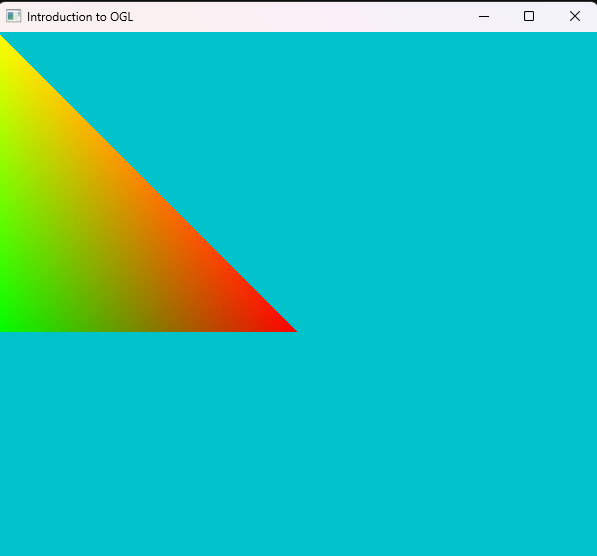
\includegraphics[width=0.6\textwidth]{Imagenes/E1/T00C2CB.png}
    \caption{Ventana OpenGL con color de fondo \#00C2CB.}
    \label{fig:fondo1}
\end{figure}

En la Figura \ref{fig:fondo2} se observa el cambio al color \#7FE0D4 (tecla 'G').\\

\begin{figure}[H]
    \centering
    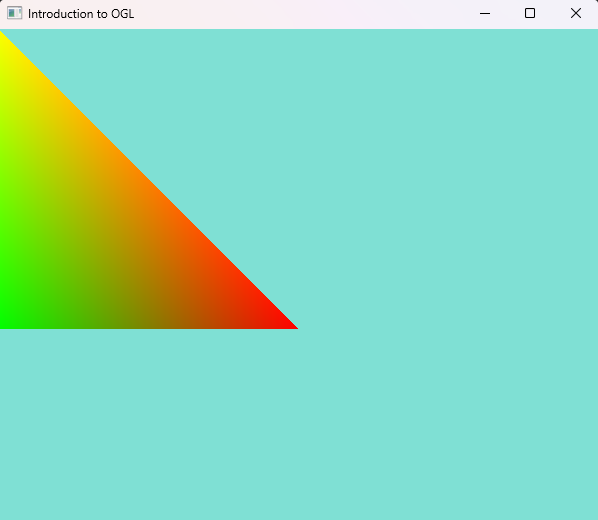
\includegraphics[width=0.6\textwidth]{Imagenes/E1/T7FE0D4.png}
    \caption{Ventana OpenGL con color de fondo \#7FE0D4.}
    \label{fig:fondo2}
\end{figure}

En la Figura \ref{fig:fondo3} se observa el cambio al color \#FFE38A (tecla 'B').\\

\begin{figure}[H]
    \centering
    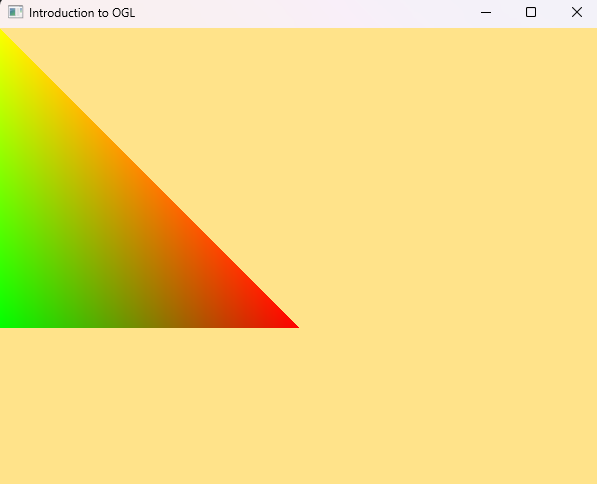
\includegraphics[width=0.6\textwidth]{Imagenes/E1/TFFE38A.png}
    \caption{Ventana OpenGL con color de fondo \#FFE38A.}
    \label{fig:fondo3}
\end{figure}

En la Figura \ref{fig:fondo4} se observa el cambio al color \#FF9A76 (tecla 'N').\\

\begin{figure}[H]
    \centering
    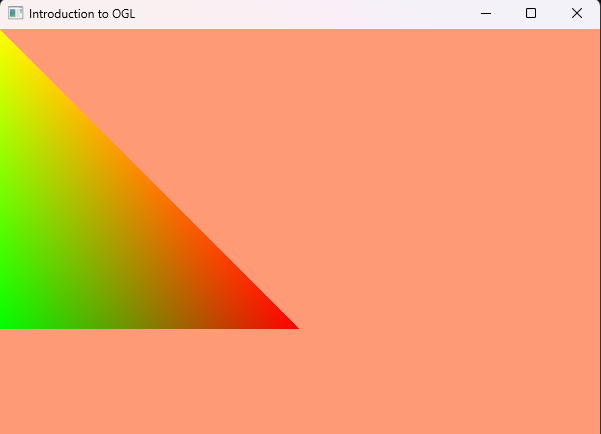
\includegraphics[width=0.6\textwidth]{Imagenes/E1/TFF9A76.png}
    \caption{Ventana OpenGL con color de fondo \#FF9A76.}
    \label{fig:fondo4}
\end{figure}

En la Figura \ref{fig:fondo5} se observa el cambio al color \#FF5D8F (tecla 'O').\\

\begin{figure}[H]
    \centering
    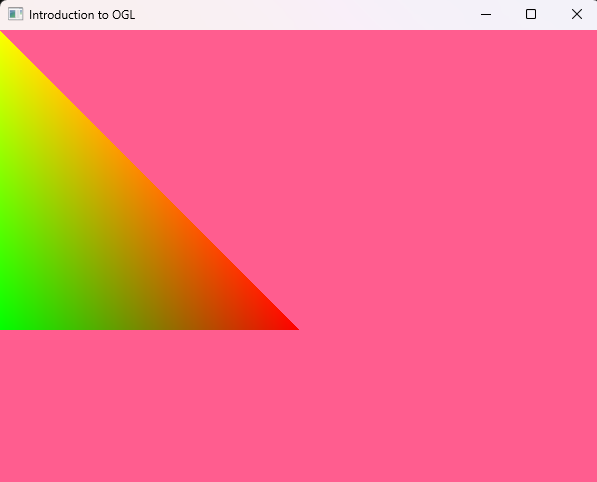
\includegraphics[width=0.6\textwidth]{Imagenes/E1/TFF5D8F.png}
    \caption{Ventana OpenGL con color de fondo \#FF5D8F.}
    \label{fig:fondo5}
\end{figure}

\subsection{Actividad 2: Rectángulo unido por dos triángulos}
Para esta actividad, se modificó la clase encargada de construir la geometría para generar un rectángulo centrado en la ventana. Se definieron cuatro vértices cuyas coordenadas en $X$ y en $Y$ se calcularon de forma simétrica a partir del origen $(0.0, 0.0)$, asegurando que la figura mantuviera una posición uniforme en el espacio normalizado. Para completar la superficie rectangular, se definieron dos triángulos en el arreglo de índices (\texttt{EBO}): el primero uniendo los vértices $0-1-2$ y el segundo conectando los vértices $0-2-3$.

A cada uno de los cuatro vértices se le asignó un color diferente de la paleta solicitada, realizando la conversión de sus valores hexadecimales al formato de punto flotante normalizado en el rango $[0.0, 1.0]$:
\begin{itemize}
    \item Vértice 0 (Superior izquierdo): \texttt{\#FF5A5F} $\rightarrow (1.000, 0.353, 0.373)$
    \item Vértice 1 (Inferior izquierdo): \texttt{\#FFB400} $\rightarrow (1.000, 0.706, 0.000)$
    \item Vértice 2 (Inferior derecho): \texttt{\#3DDC84} $\rightarrow (0.239, 0.863, 0.518)$
    \item Vértice 3 (Superior derecho): \texttt{\#00A6ED} $\rightarrow (0.000, 0.651, 0.929)$
\end{itemize}

Al momento de ejecutar el programa, el \textit{Fragment Shader} generó una interpolación bilineal por toda la superficie del rectángulo, mostrando la transición entre los cuatro colores. A continuación, se muestra el resultado.

\begin{figure}[H]
    \centering
    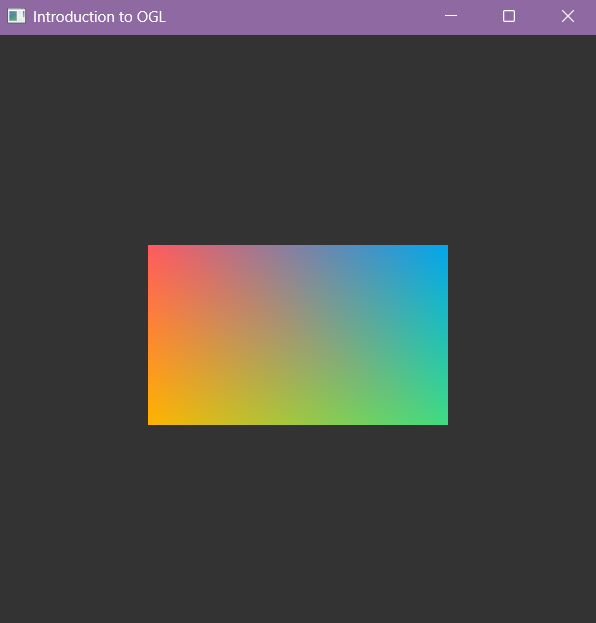
\includegraphics[width=0.5\textwidth]{Practicas/P1/Imagenes/E1/rectangulo1.png}
    \caption{Ventana OpenGL con el rectángulo.}
    \label{fig:rectangulo1}
\end{figure}

Ahora se muestra el mismo rectángulo pero con el fondo de color azul:

\begin{figure}[H]
    \centering
    \includegraphics[width=0.5\textwidth]{Practicas/P1/Imagenes/E1/rectangulo1.2.png}
    \caption{Ventana OpenGL con el rectángulo y fondo azul.}
    \label{fig:rectangulo1.2}
\end{figure}

\subsection{Actividad 2.1: Rectángulo unido por dos triángulos (Variación)}

Como variación, se adaptaron las dimensiones del rectángulo para que se proyectara con una orientación vertical en lugar de horizontal, conservando su posición centrada en $(0.0, 0.0)$. Asimismo, se cambió el color del vértice superior derecho por el tono morado (\texttt{\#8B5CF6} $\rightarrow (0.545, 0.361, 0.965)$), integrando así el quinto color de la paleta. Adicionalmente, se modificó el orden de conexión de los índices a $0-1-3$ y $1-2-3$ para cambiar la dirección de la diagonal compartida por ambos triángulos.

\begin{figure}[H]
    \centering
    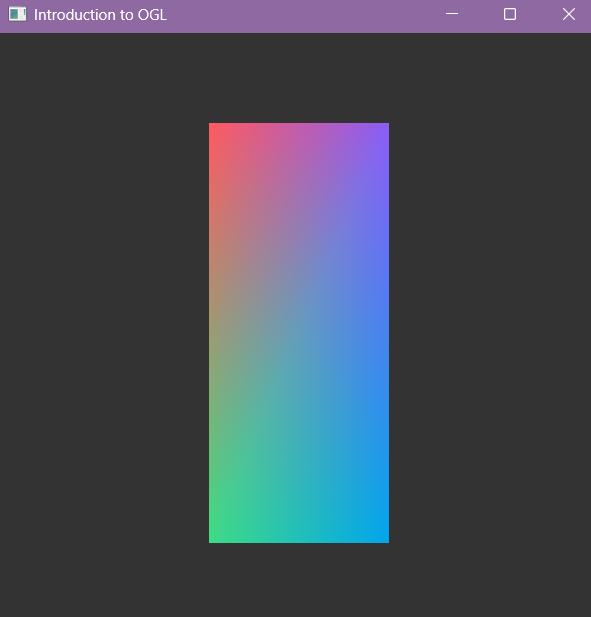
\includegraphics[width=0.45\textwidth]{Practicas/P1/Imagenes/E1/Rectangulo2.png}
    \caption{Ventana OpenGL con el rectángulo vertical.}
    \label{fig:rectangulo2}
\end{figure}

Ahora se muestra el mismo rectángulo pero con el fondo de color azul:

\begin{figure}[H]
    \centering
    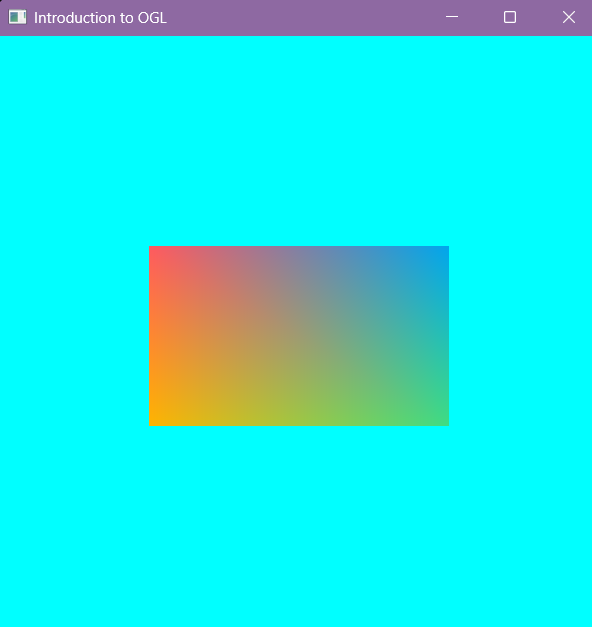
\includegraphics[width=0.45\textwidth]{Practicas/P1/Imagenes/E1/Rectangulo1.2.png}
    \caption{Ventana OpenGL con el rectángulo vertical y fondo azul.}
    \label{fig:rectangulo1.2}
\end{figure}